\subsection{Optika}
 \todo{}

V tejto kapitole si ukážeme prekvapivý súvis Fourierovej transformácie
s fyzikálnym javom nazývaným interferencia svetla. Aby sme sa však
dopracovali k tomuto výsledku, musíme najskôr prejsť sadou definícií a
viet.

Vo všeobecnoti, fyzikálny pojem interferencia vĺn je fenomén, ktorý
nastáva, keď sa dve (alebo viac) vlny putujúce spoločným médiom
stretnú. Nech $A(r,t)$ je amplitúda prvej vlny na mieste $r$ v čase $t$.
Podobne, nech $B(r,t)$ je amplitúda druhej vlny.

Podľa princípu superpozície (Huygensovho princípu) je výsledkom
spoločného putovania vĺn A,B vlna C, pre ktorú platí
 $C(r,t)=A(r,t)+B(r,t)$. Názorná ukážka skladania vĺn je na obrázku
 \ref{fig:interferencia}.
Princíp superpozície a interferencia vôbec sa vo
 fyzike používa na viacerých miestach a to najmä v kvantovej fyzike.

 \begin{figure}[htp]
 \centering
 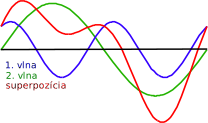
\includegraphics{obrazky/optika/interferencia_1}
 
\includegraphics{obrazky/optika/interferencia_2}

 \caption{Interferencia 2 vĺn a) na priamke b) na ploche}
 \label{fig:interferencia}
 \end{figure}

Pre jednoduchosť budeme uvažovať interferenciu monochromatických vĺn.
Prax ukazuje, že zaujímavá vie byť aj všeobecná interferencia,
napríklad farebné sfarbenie povrchu bublín či olejových škvŕn, ale
táto téma je už nad rámec tejto publikácie.

Zoberme teda zdroj (skalárneho) vlnenia v 3-rozmernom priestore.
Ak je poloha zdroja $\vect{a}$, amplitúda $A$, počiatočná fáza $\phi$ a vlnová dĺžka
$\lambda$, tak v čase $t$ bude v mieste $\vect{r}$ výsledná amplitúda rovná

\begin{equation}
X(\vect{r},t)=A \sin(2 \pi \frac{|\vect{r}-\vect{a}| - t c}{\lambda}+\phi)
\end{equation}

Podľa princípu superpozície pre $N$ zdrojov $1,\dots,N$ platí
\begin{equation}
X(\vect{r},t)=\sum_{i=1}^{N} A_i \sin(2 \pi
\frac{|\vect{r}-\vect{a_i}| - t c}{\lambda}+\phi_i)
\end{equation}

Na tomto mieste si povieme niečo o objektoch zvaných komplexné
amplitúdy.

\definicia{Komplexná amplitúda}{
Nech má vlna amplitúdu $A$ a fázu $\phi$.
Pod pojmom komplexná amplitúda budeme rozumieť komplexné číslo
$\mathcal{A}=A e^{i \phi}$.
}


Lema: Reálna časť komplexnej amplitúdy je amplitúda vlny v danom bode.
Dôkaz: Komplexná amplitúda je vlastne obohatenie pôvodného vzorca o
imaginárnu časť.


Lema: Energia prislúchajúca vlne je $E \thickapprox A^2$.

Definicia: Nech $a$ je amplitúda vlny s periódou $p$. 
Potom priemerná energia $E_p \thickapprox \frac{1}{p} \int_0^p a(x)^2 dx$.

\begin{poznamka}
 Našim cieľom bude zhodnotiť energiu rýchlo kmitajúcej vlny.
 Čitateľ si tak môže všimnúť analógiu tohoto deja s elektrickou
 energiou. Keď máme jednosmerný obvod, energia ktorá sa spotrebúva
 napríklad na rezistore je časovo konštantná. Naproti tomu za
 prítomnosti striedavého napätia táto energia (za jednotku času) kolíše
 a v praxi nás zaujíma len jej stredná hodnota. To isté môžeme
 uvažovať aj u svetla, kedy nás nezaujíma energia (resp.
 pravdepodobnosť výskytu fotónov z kvantovej mechaniky) 
 na danom mieste v konkrétnom čase,
 ale jej stredná hodnota, lebo to je veličina ktorú vieme merať.
\end{poznamka}

Veta: Priemerná energia sínusovej vlny s komplexnou amplitúdou
$\mathcal{A}$ $E_p \thickapprox |\mathcal{A}|^2$.
Dôkaz:
$E_p \thickapprox \frac{c}{\lambda} \int_0^{\lambda/c}
(A \sin(2 \pi \frac{L - t c}{\lambda}+\phi))^2
= A^2 \frac{c}{\lambda} \frac{\lambda}{2 c} =
\frac{1}{2} A^2 = \frac{1}{2} \mathcal{A}^2$.

\todo{pokracovanie}
